\section{Simulation du système}

Nous nous intéresserons maintenant au système complet afin de simuler les différentes réponses aux évènements tels que step sur $DV$, step sur $SP$ ou activation du feedforward, et ce, dans les conditions réelles des futures réponses expérimentales.

Il est bon de rappeler que tout ce qui va être simulé sera fait autour d'un point de fonctionnement, et valable uniquement aux alentours de ce point.
Dans notre cas, nous avons la puissance de chauffe du premier radiateur $MV_0 = 50\%$, la puissance de chauffe du deuxième radiateur $DV_0 = 50\%$ et la sortie du système en régime permanent $PV_0 = 49.3^{\circ}$C.

Pour l'instant, le paramètre $\alpha$ sera fixé à $\alpha = 1$ par simplicité et $\gamma$ sera fixé à $\gamma = 0.7$ pour éviter une réponse du régulateur trop aggressive.
On utilisera les paramètres optimaux du second ordre trouvés à la Section 2 \textit{Identification de la Dynamique} pour simuler le Processus et la Perturbation.

\noindent Nous alons ici analyser les scénarios suivants :
\begin{enumerate}
    \item Réponse en mode \underline{manuel} (boucle ouverte) \underline{sans} FeedForward
    \item Réponse en mode \underline{manuel} (boucle ouverte) \underline{avec} FeedForward
    \item Réponse en mode \underline{automatique} (boucle fermée) \underline{sans} FeedForward
    \item Réponse en mode \underline{automatique} (boucle fermée) \underline{avec} FeedForward
\end{enumerate}

\subsection{Réponse à une perturbation \texorpdfstring{$DV$}{DV} en mode manuel sans FF}
\begin{figure}[H]
    \centering
    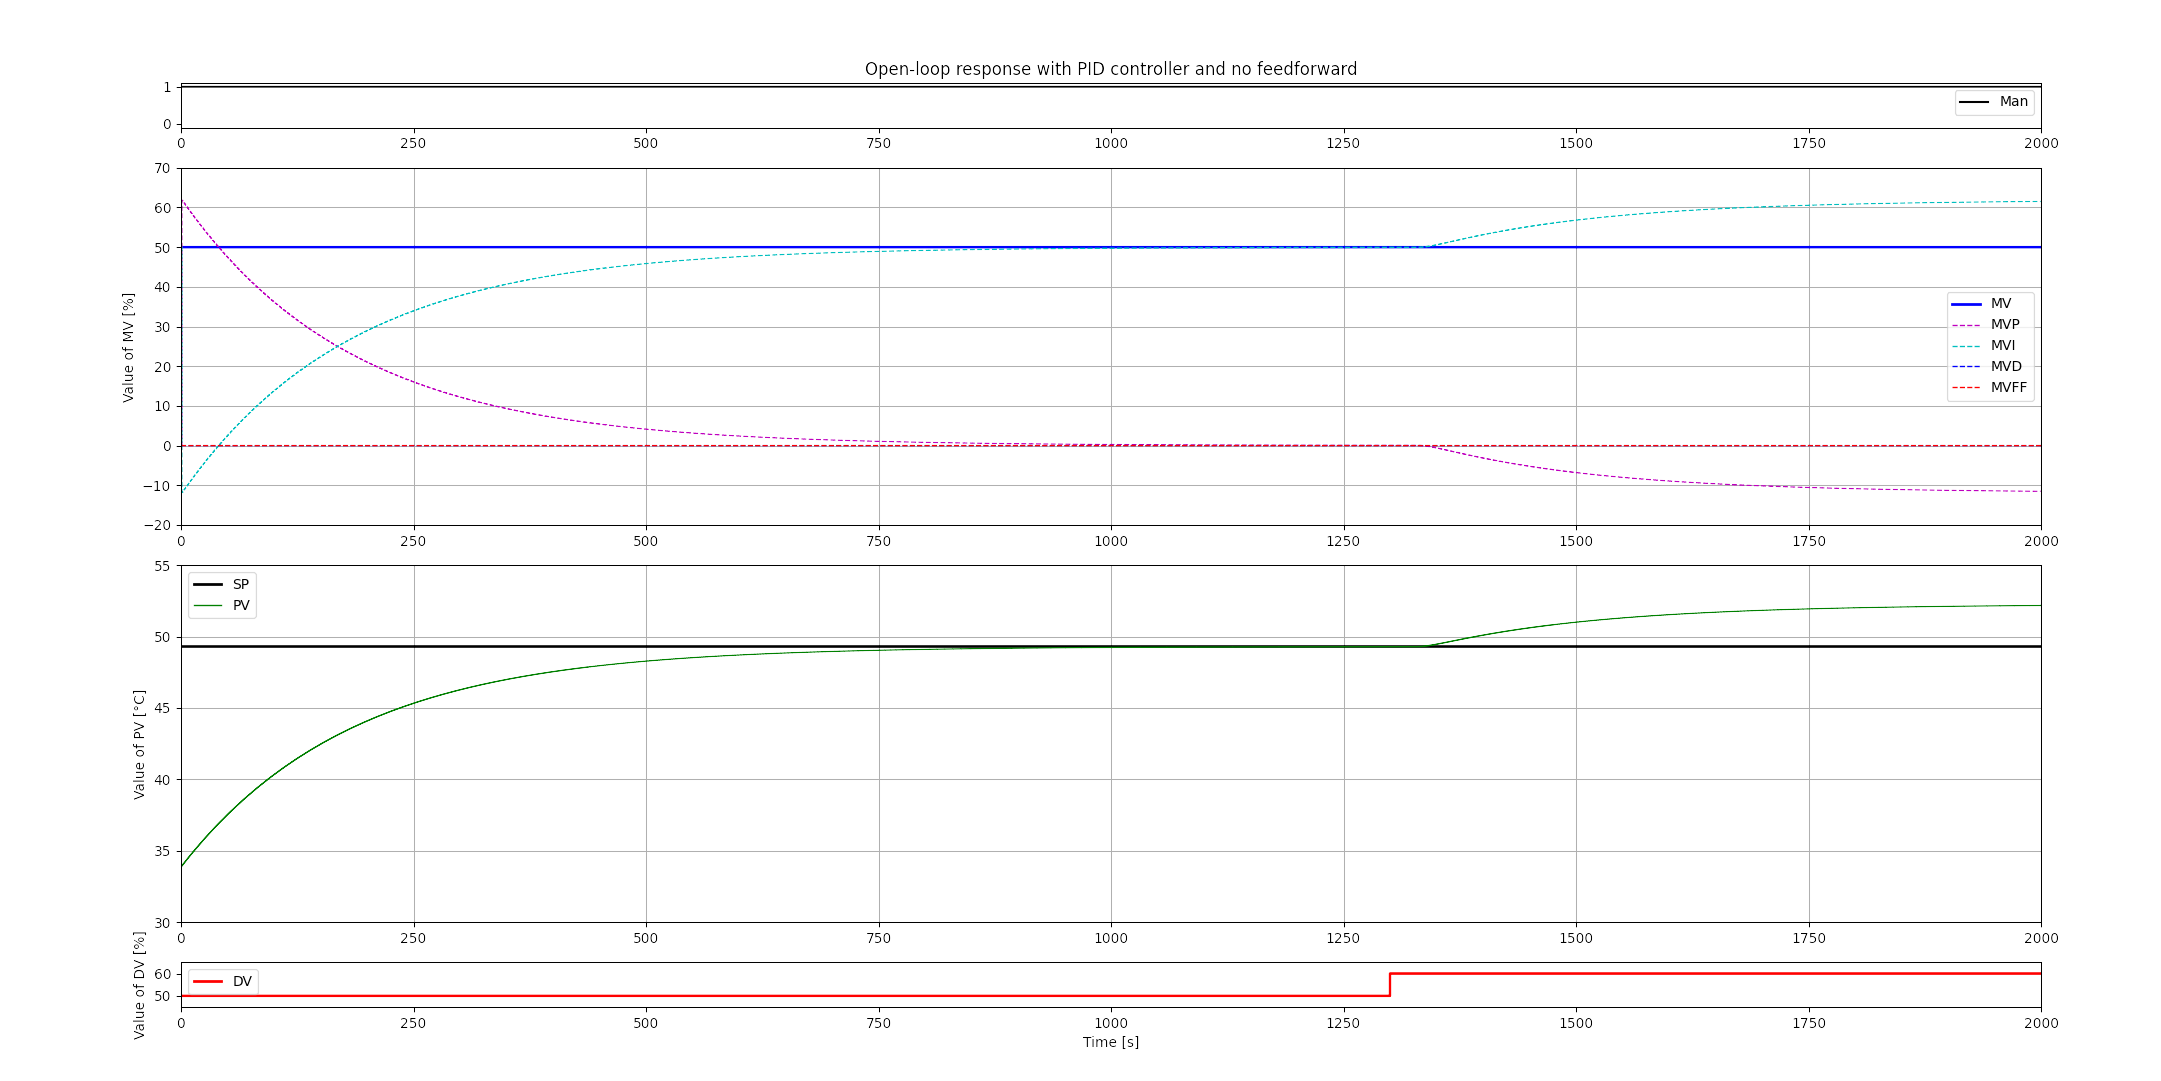
\includegraphics[width=0.9\textwidth]{../Plots/Simulation_scenario_2.png}
    \caption{Réponse à boucle ouverte sans FeedForward}
    \label{fig:Simulation_OLP_no_FF}
\end{figure}
La Figure \ref{fig:Simulation_OLP_no_FF} confirme bien que l'on est en mode manuel en imposant une valeur de $MV = MV_0$.
Il est dès lors logique de voir l'action intégrale $MV_I$ s'adapter tout le long de la simulation en raison du Reset de l'Action Intégrale.\\
Nous constatons que l'action dérivée $MV_D$ est nulle, ce qui est normal étant donné que la constante de temps $T_D$ est nulle. Notre processus agit comme un premier ordre et donc notre régulateur est assimilé à un régulateur PI.

L'action proportionnelle $MV_P$ fait un pic au début de la simulation. Cela est dû à la différence entre la consigne et la sortie du système, donc l'erreur.
En effet, la composante proportionnelle est directement proportionnelle à l'erreur et au gain statique : $MV_P = K_C \, E \approx 4 \cdot 15\% = 60\%$.\\
La sortie de processus $PV$ met alors un certain temps à se stabiliser autour de la valeur de consigne $SP = PV_0$ (temps d'établissement).

Une perturbation est alors appliquée. Le feedforward étant désactivé, elle se trouve répercutée sur $PV$.
Comme attendu, cette variation introduit une erreur négative que l'on voit sur $MV_P$. Le reset de l'action intégrale fait son travail en venant augmenter $MV_I$ afin de conserver la valeur manuelle de $MV$.\\
Il est également intéressant de retrouver le délai en regardant la différence entre le moment où la perturbation est appliquée et le moment où $PV$ réagit.

\subsection{Réponse à une perturbation \texorpdfstring{$DV$}{DV} en mode manuel avec FF}
\begin{figure}[H]
    \centering
    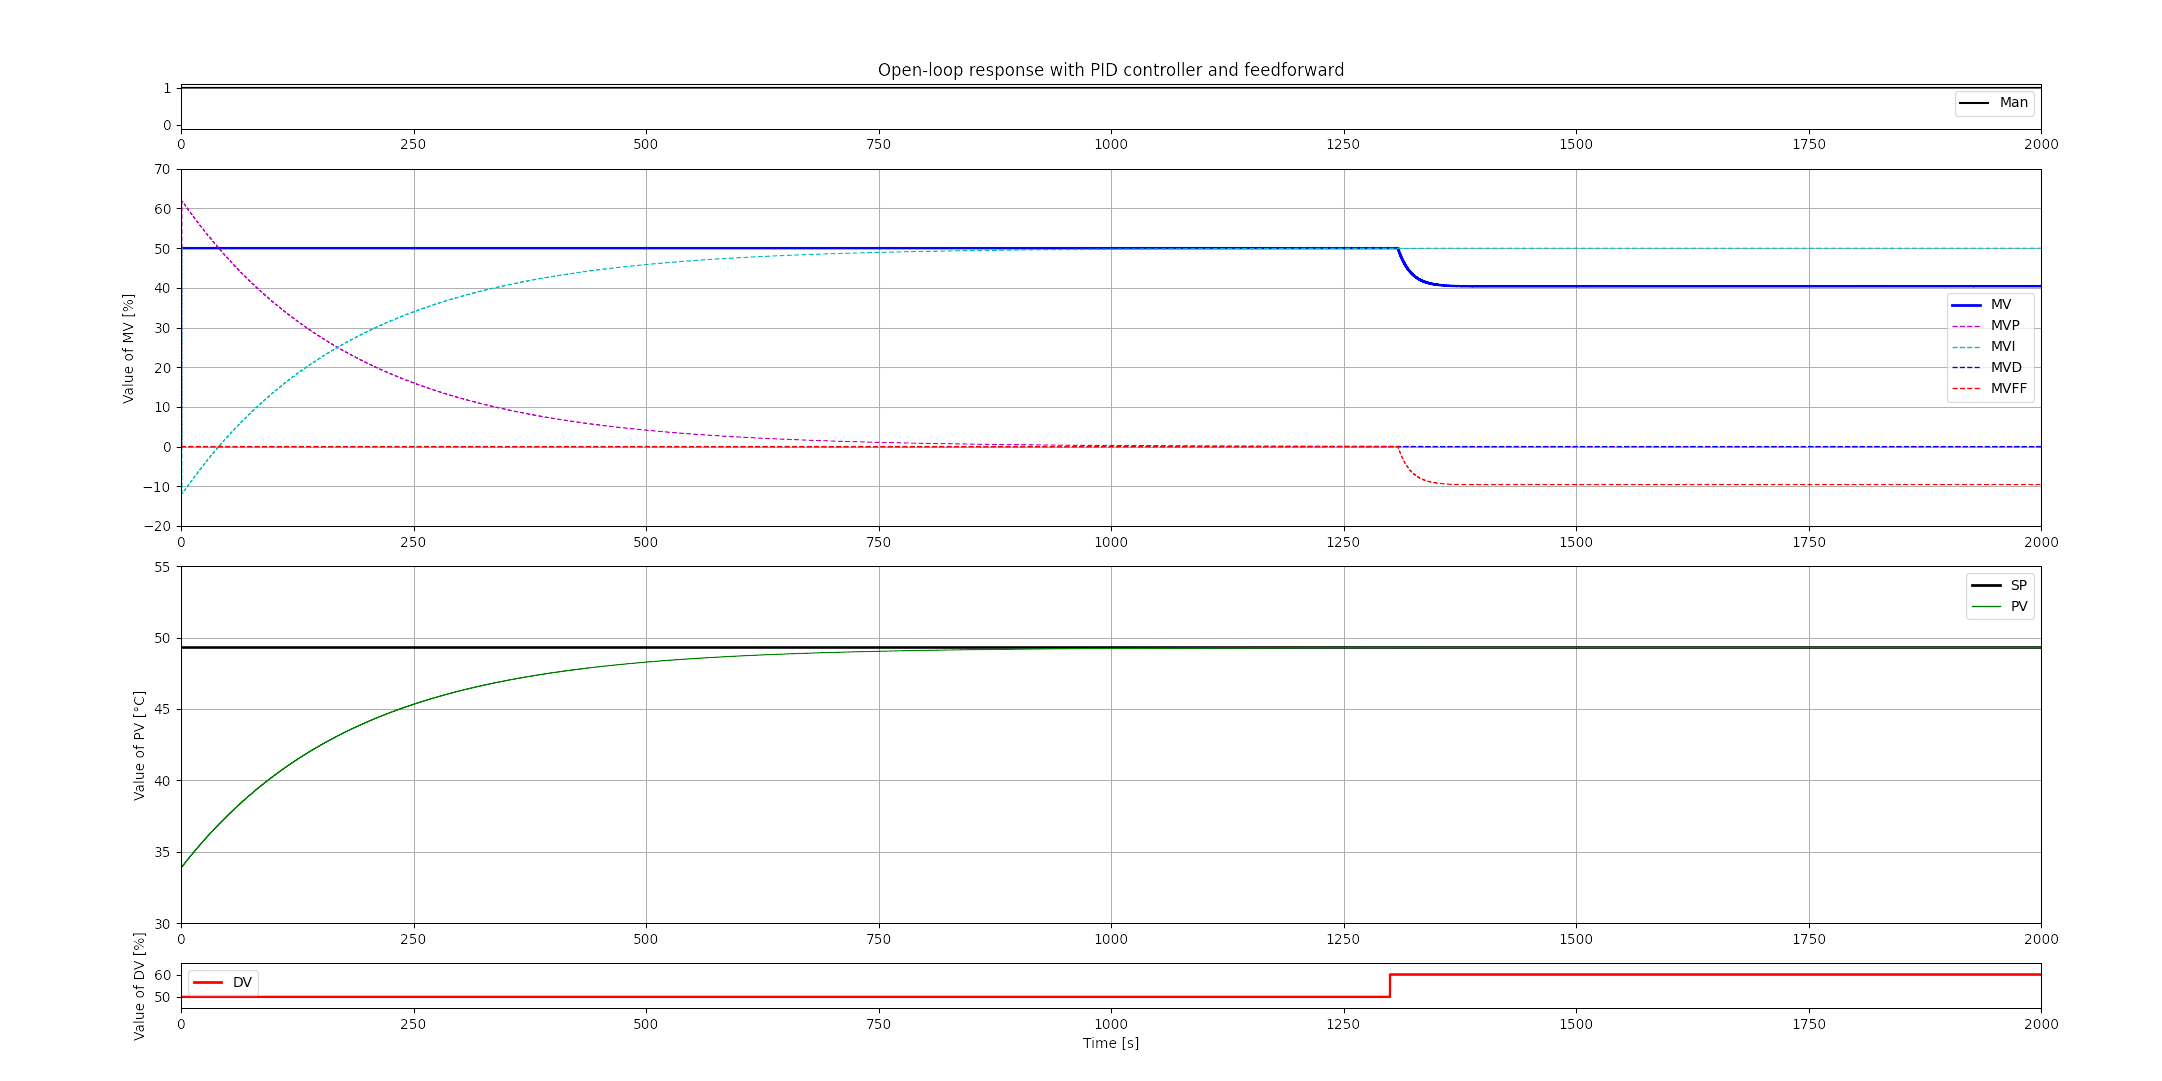
\includegraphics[width=0.9\textwidth]{../Plots/Simulation_scenario_3.png}
    \caption{Réponse à boucle ouverte avec FeedForward}
    \label{fig:Simulation_OLP_FF}
\end{figure}
Dans ce scénario, le feedforward est activé. La perturbation $DV$ est donc prise en compte anticipativement.
Nous constatons que la composante $MV_{FF}$ réagit bien comme attendu à la perturbation. $MV$ est donc lui même ajusté pour compenser la perturbation et ainsi conserver $PV = SP = PV_0$.\\
Encore une fois, nous pouvons nous intéresser au délai qui se trouve maintenant réduit puisqu'il s'agit du délai du feedforward $\theta_{FF} = \theta_D - \theta_P = 29 - 20 = 9\,s$.

\subsection{Réponse à une perturbation \texorpdfstring{$DV$}{DV} \& changement de consigne \texorpdfstring{$SP$}{SP} en mode automatique sans FF}
\begin{figure}[H]
    \centering
    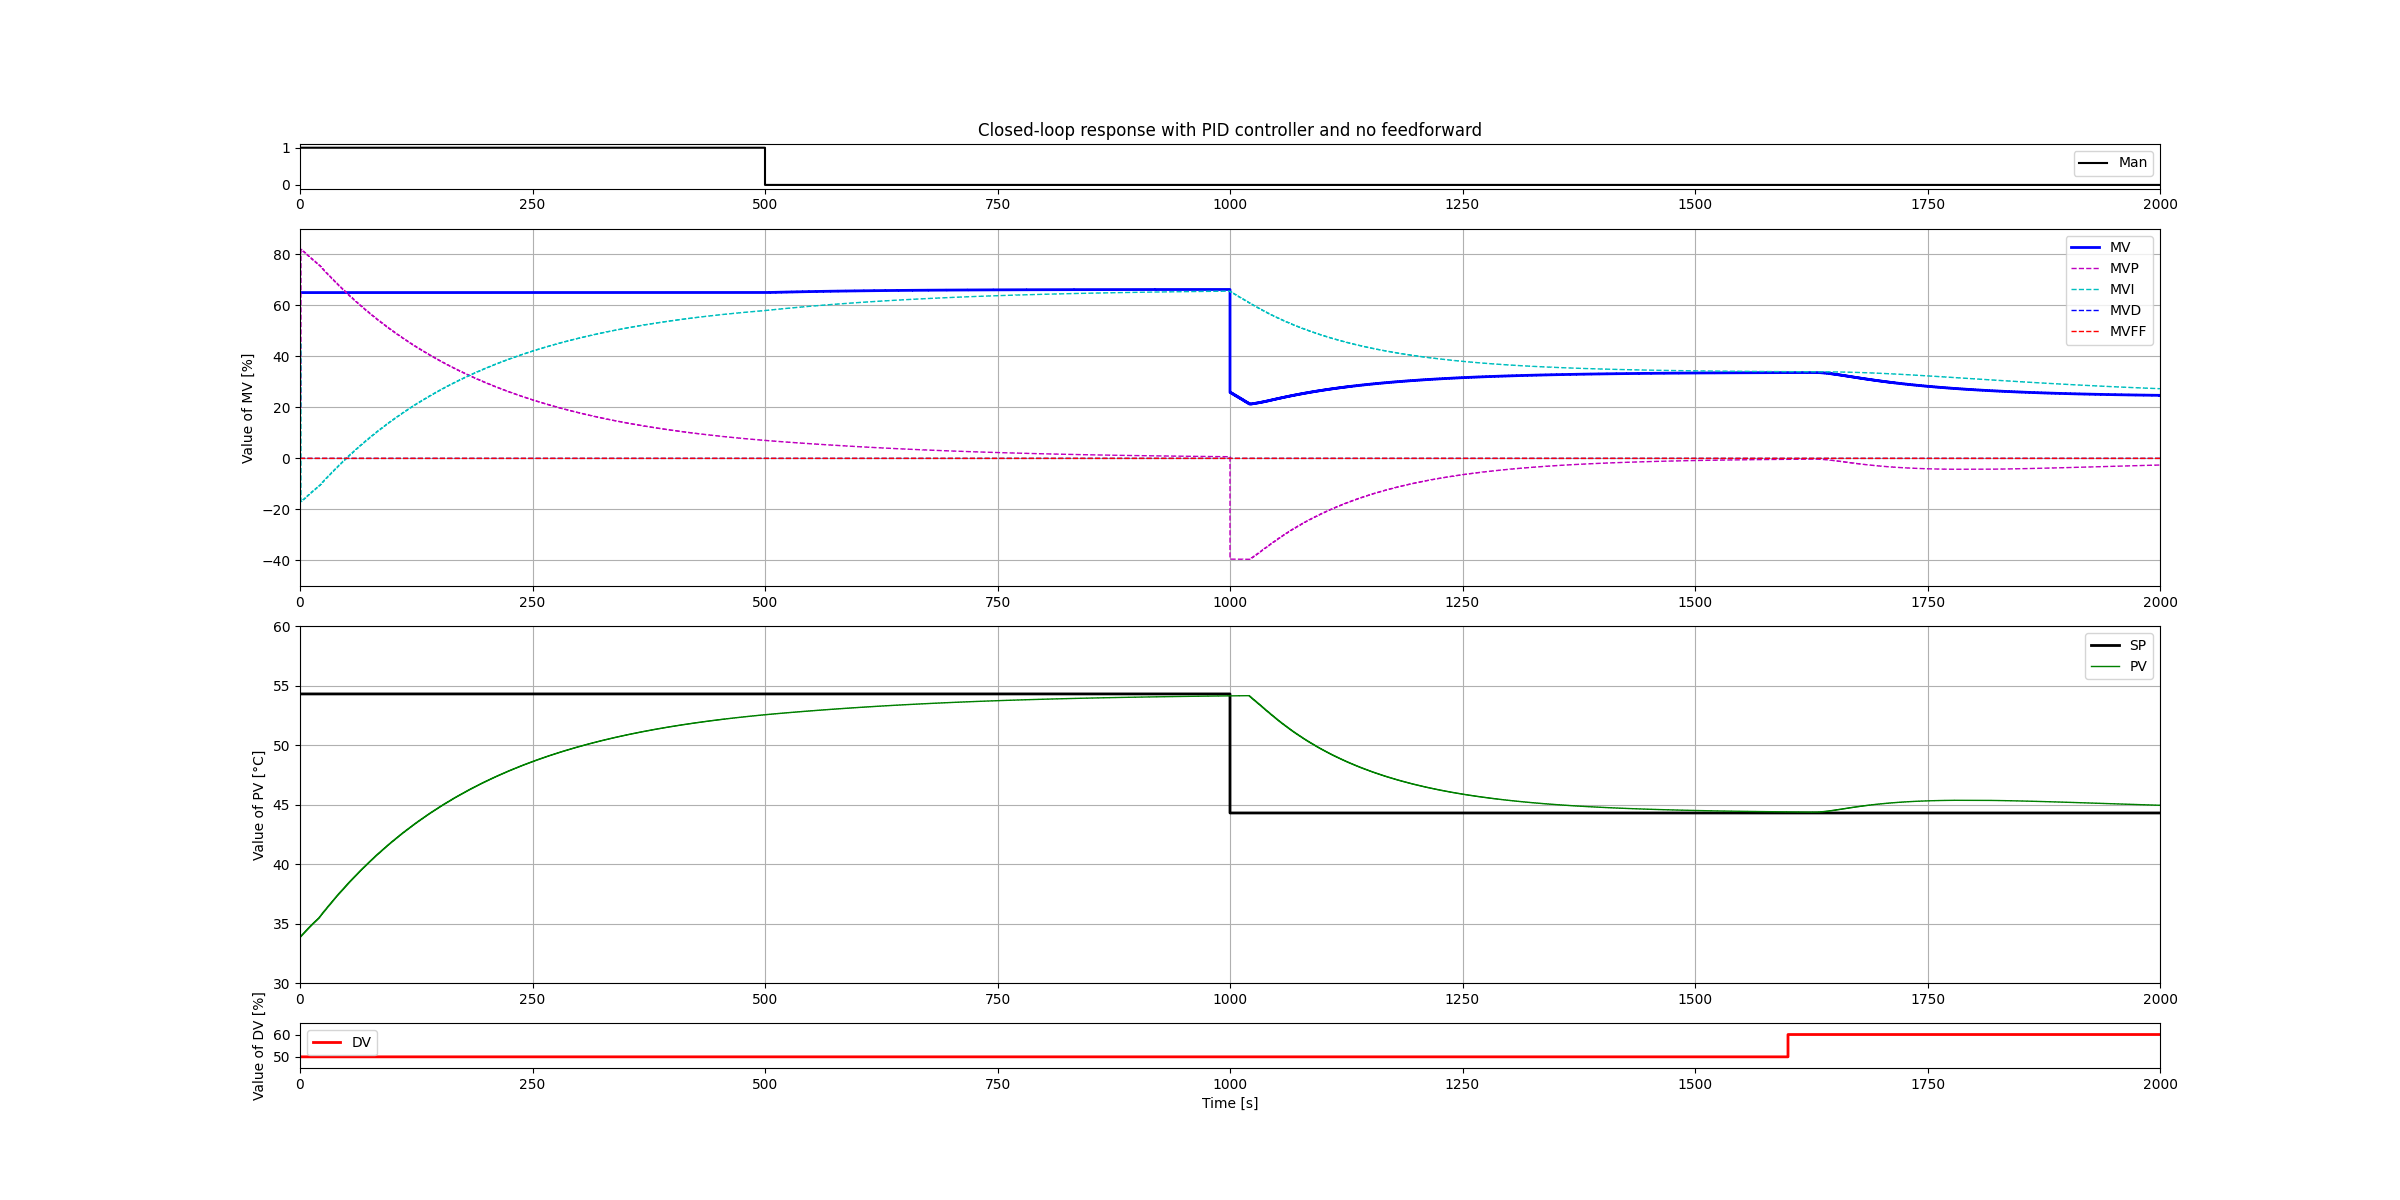
\includegraphics[width=0.9\textwidth]{../Plots/Simulation_scenario_5.png}
    \caption{Réponse à boucle fermée sans FeedForward}
    \label{fig:Simulation_CLP_no_FF}
\end{figure}
La Figure \ref{fig:Simulation_CLP_no_FF} utilise le mode manuel les quelques 500 premières secondes le temps d'amener $PV$ suffisement proche de $SP$, le mode automatique se charge de stabiliser $PV$.\\
On remarque tout de suite la réponse de $MV$ sur le step de $SP$, qui forme un pic avec un angle.
Nous pouvons enfait expliquer cela par la présence notable du délai $\theta_P = 20\,s$ entre $SP$ et $PV$.
En introduisant une erreur négative, l'action proportionnelle $MV_P = K_C \, E$ diminue mais l'erreur ne commencera à être compensée que après un délai $\theta_P$.
L'action intégrale $MV_I$, elle, diminue progressivement dès lors qu'elle accumule une erreur négative, faisant apparaître cette forme particulière sur $MV$.

Sans feedforward et comme mentionné précedement, une perturbation est bien relfetée sur $PV$.
$MV_P$ va suivre l'erreur introduite et automatiquement diminuer $MV$.
Encore une fois, l'action intégrale accumule cette erreur négative permettant à $MV$ de se stabiliser à une puissance de chauffe et ainsi faire retourner petit à petit $PV$ à la consigne $SP$.

\subsection{Réponse à une perturbation \texorpdfstring{$DV$}{DV} \& changement de consigne \texorpdfstring{$SP$}{SP} en mode automatique avec FF}
\begin{figure}[H]
    \centering
    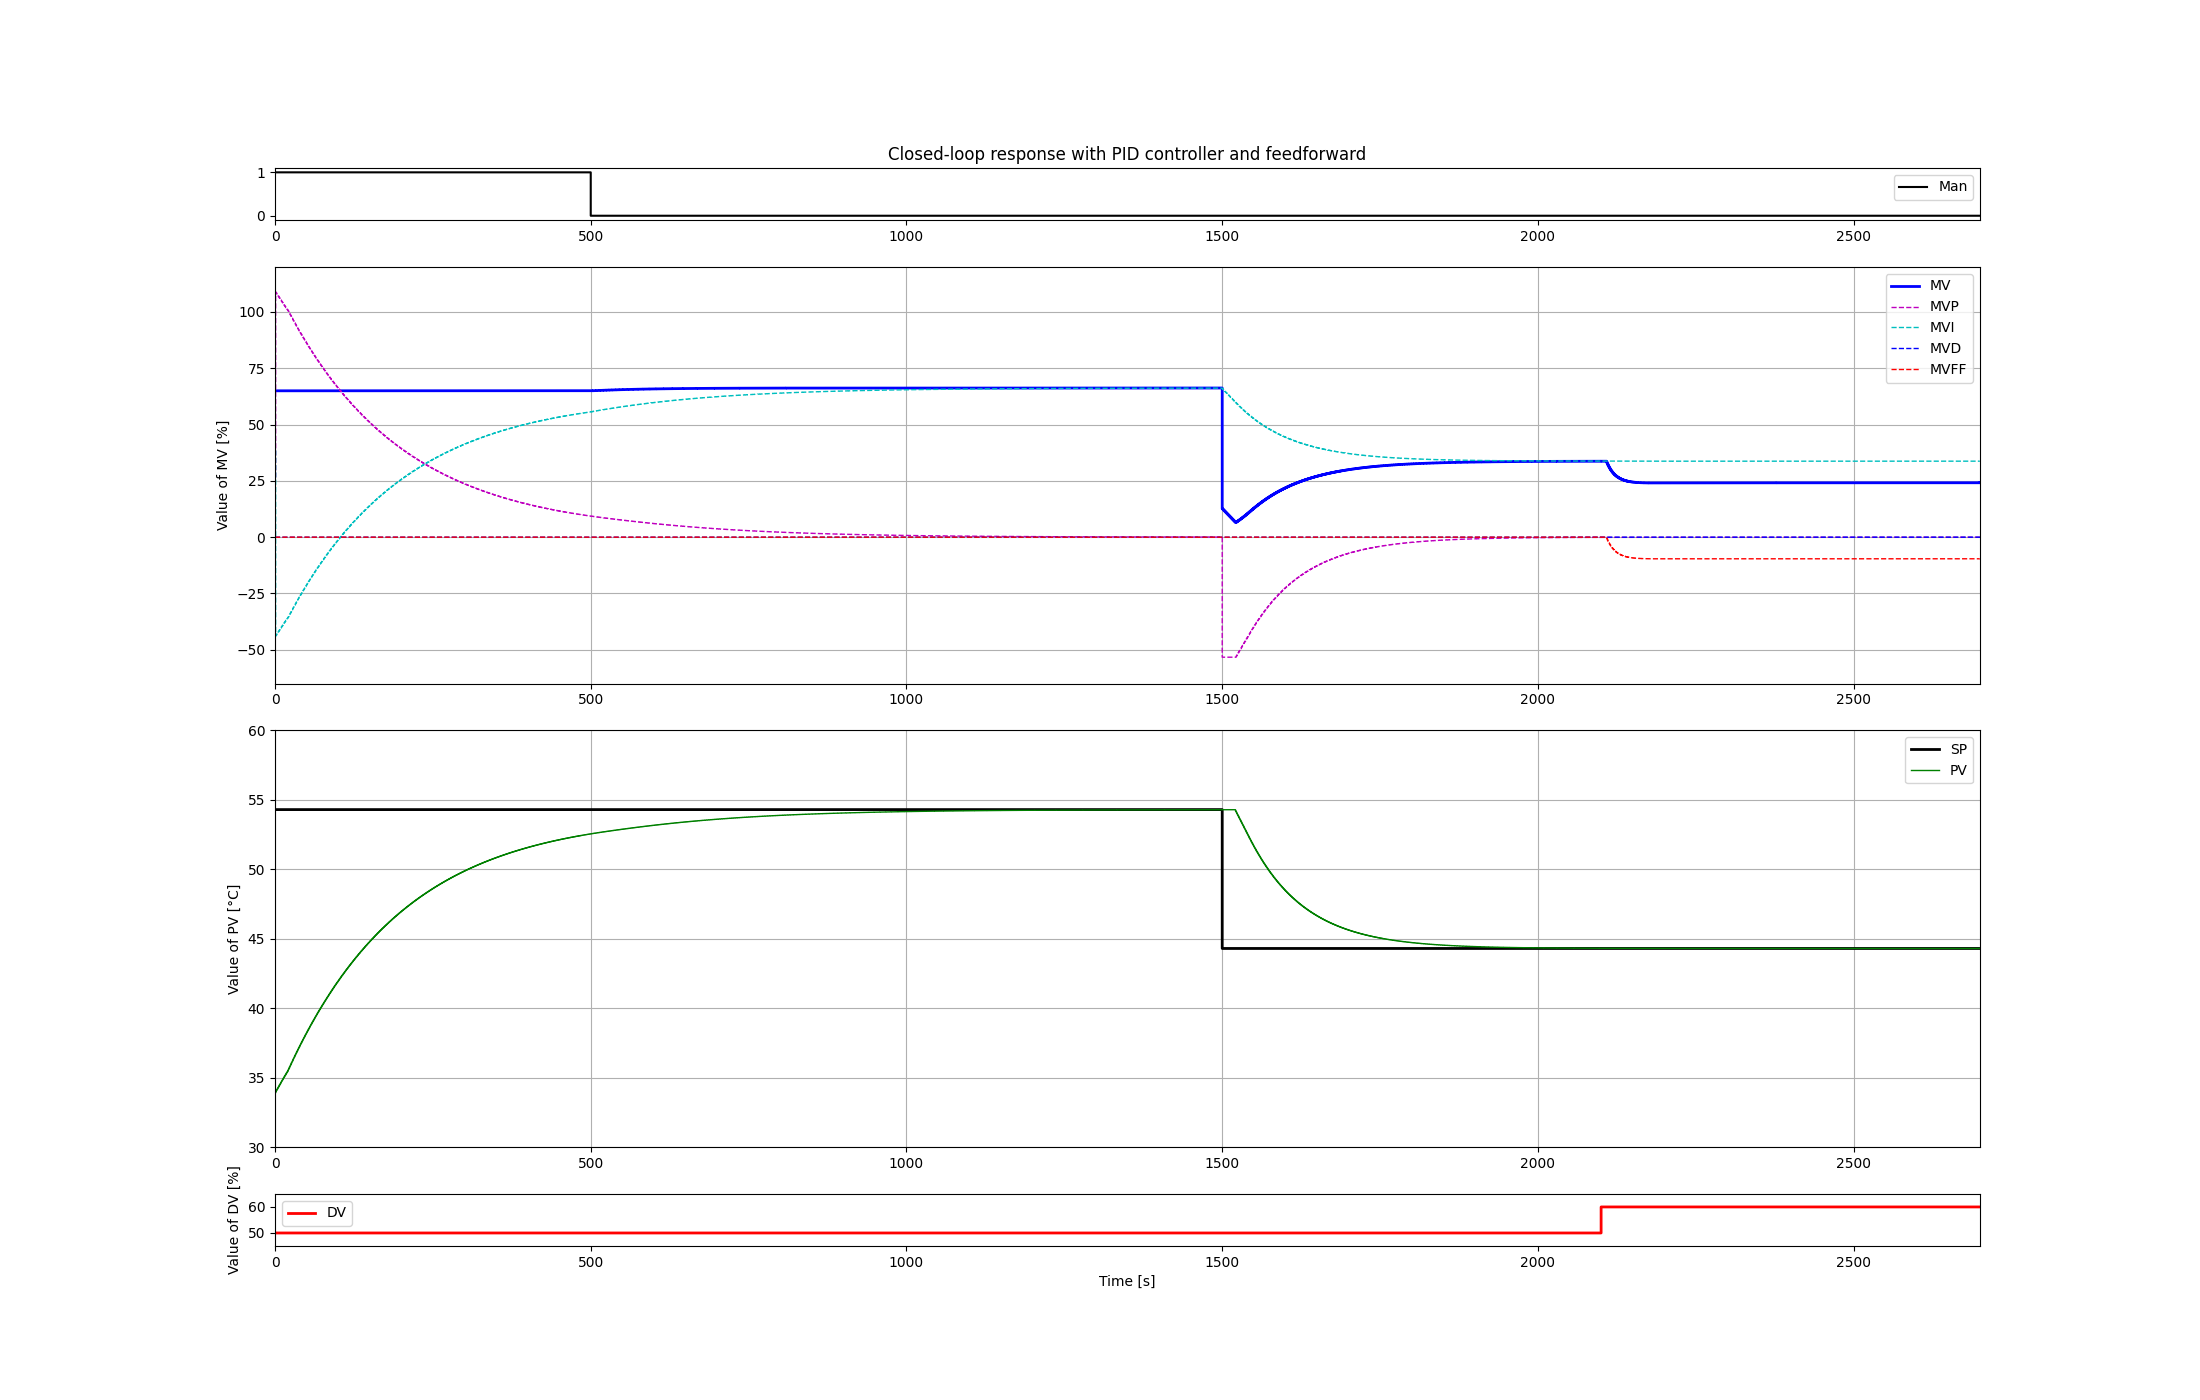
\includegraphics[width=0.9\textwidth]{../Plots/Simulation_scenario_7.png}
    \caption{Réponse à boucle fermée avec FeedForward}
    \label{fig:Simulation_CLP_FF}
\end{figure}
Sur la Figure \ref{fig:Simulation_CLP_FF} est représenté tout ce qui a été dit précedement notamment l'anticipation de la perturbation par le feedforward lorsque $MV_{FF}$ est diminué.
Encore une fois, le délai entre perturbation $DV$ et le feedforward $MV_{FF}$ est réduit à $\theta_{FF} = 9\,s$.

\subsection{Influence de \texorpdfstring{$\alpha$}{alpha} et \texorpdfstring{$\gamma$}{gamma}}
\begin{figure}[H]
    \centering
    \begin{subfigure}[b]{0.48\textwidth}
        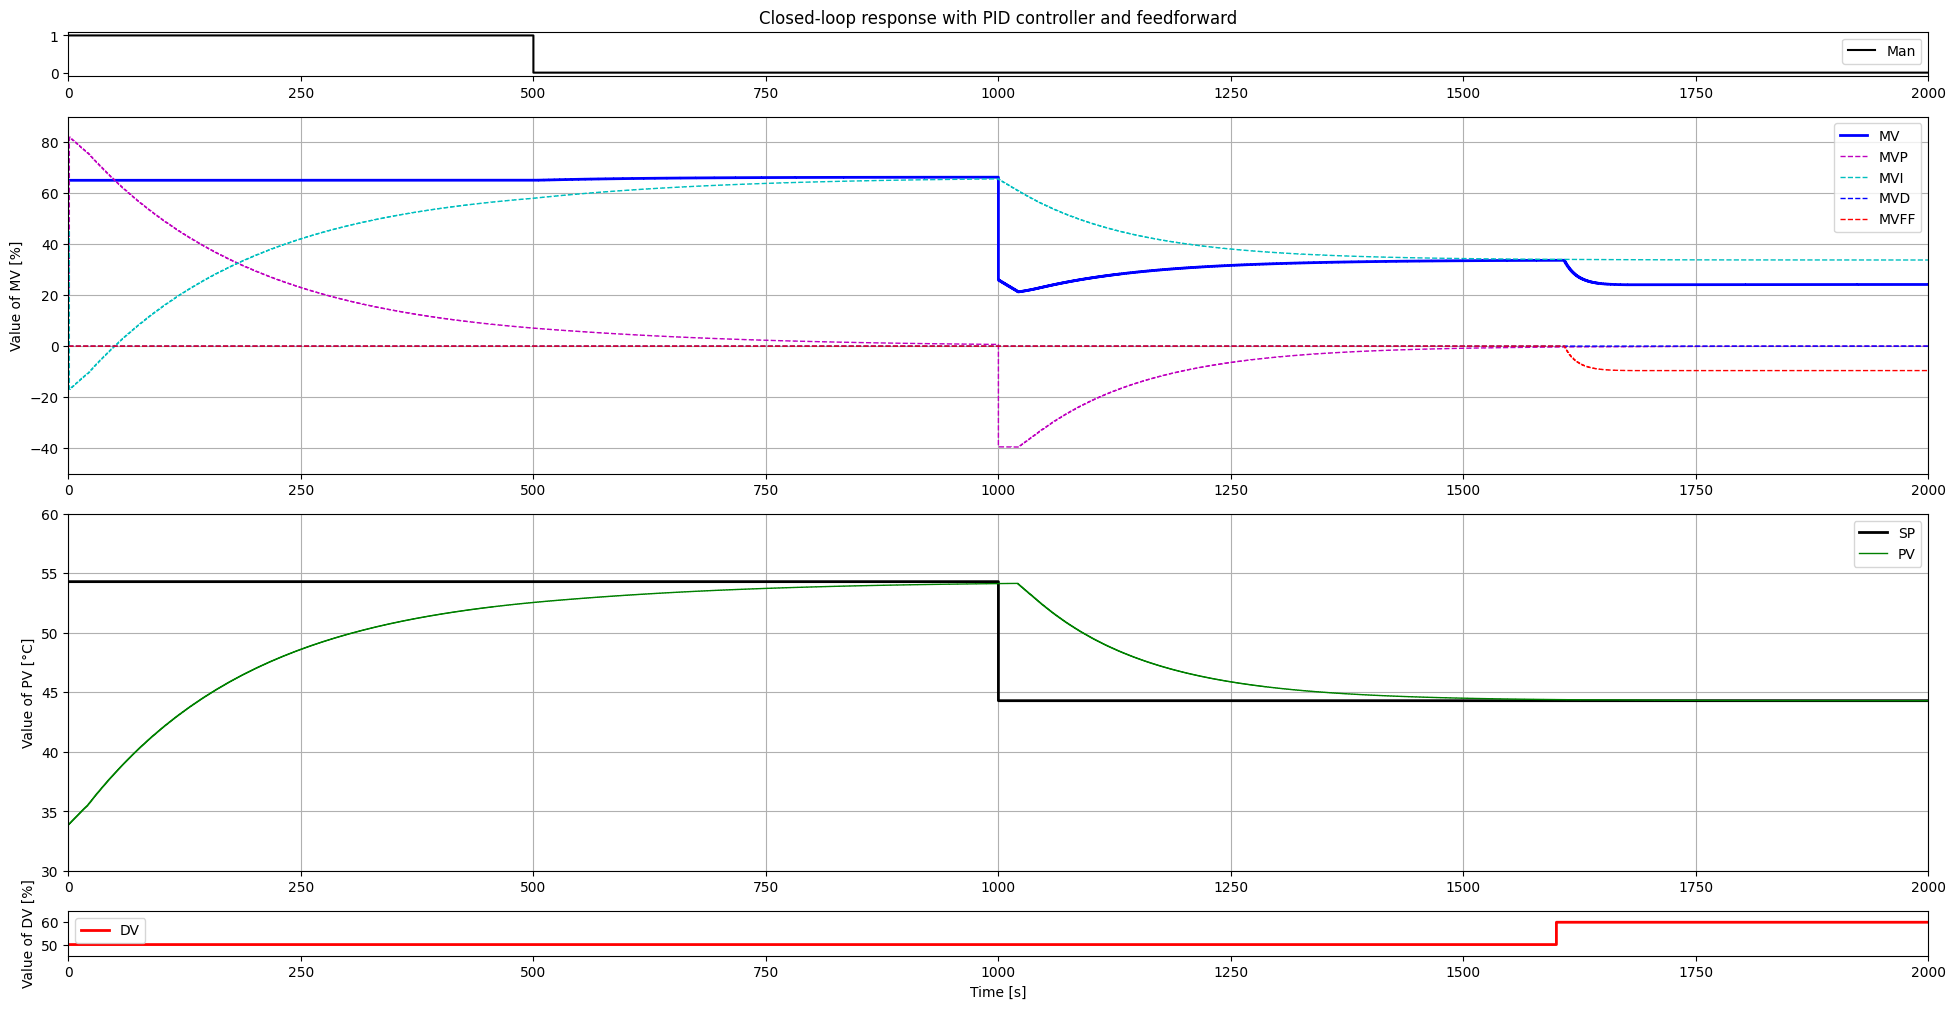
\includegraphics[width=\textwidth]{../Plots/Simulation_scenario_7_alpha=0.2.png}
        \caption{$\alpha = 0.2$}
    \end{subfigure}
    \begin{subfigure}[b]{0.48\textwidth}
        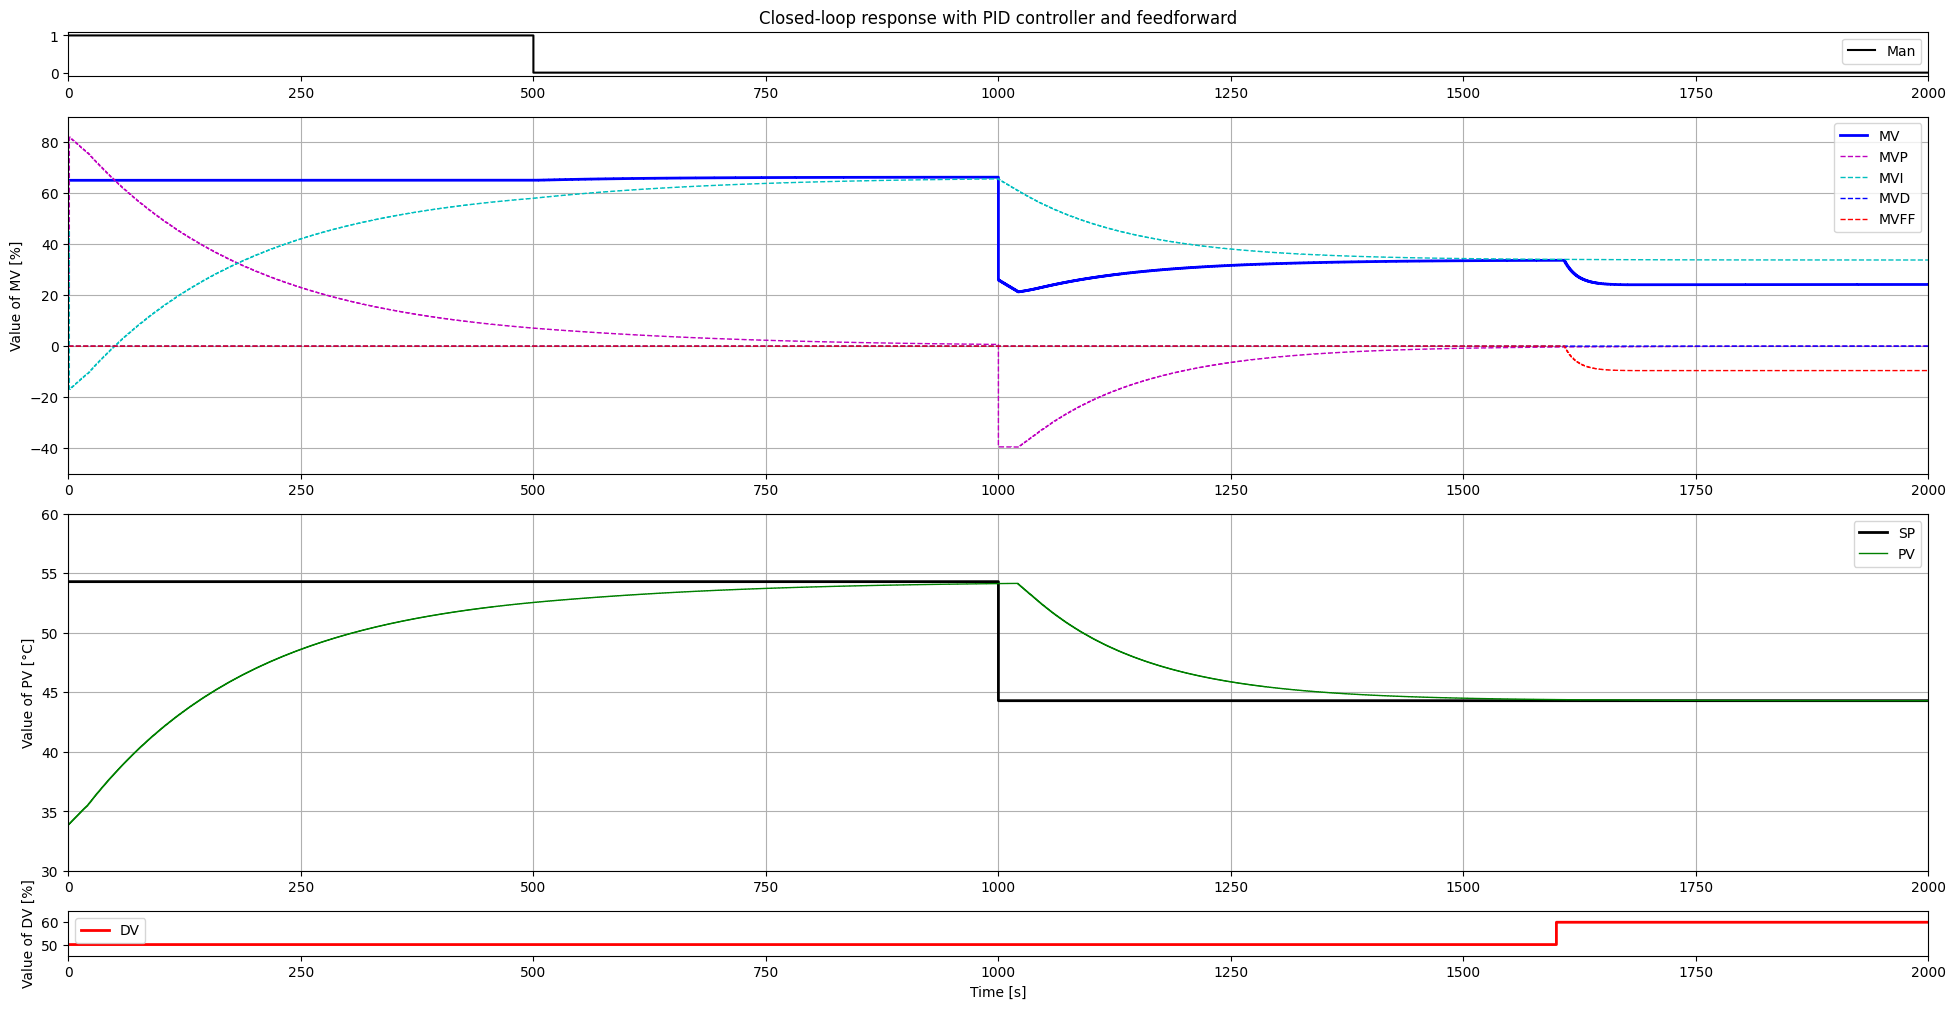
\includegraphics[width=\textwidth]{../Plots/Simulation_scenario_7_alpha=1.png}
        \caption{$\alpha = 1$}
    \end{subfigure}
    \caption{Influence de $\alpha$ sur la boucle fermée}
    \label{fig:Simulation_alpha_influence}
\end{figure}
La Figure \ref{fig:Simulation_alpha_influence} permet de montrer que, \underline{pour notre système}, $\alpha$ n'a aucune influence.
Il n'intervient que dans la limitation du gain haute fréquence de l'action dérivée. Or notre régulateur agit comme un régulateur PI, donc l'action dérivée reste nulle tout le long de la simulation.

\begin{figure}[H]
    \centering
    \begin{subfigure}[b]{0.48\textwidth}
        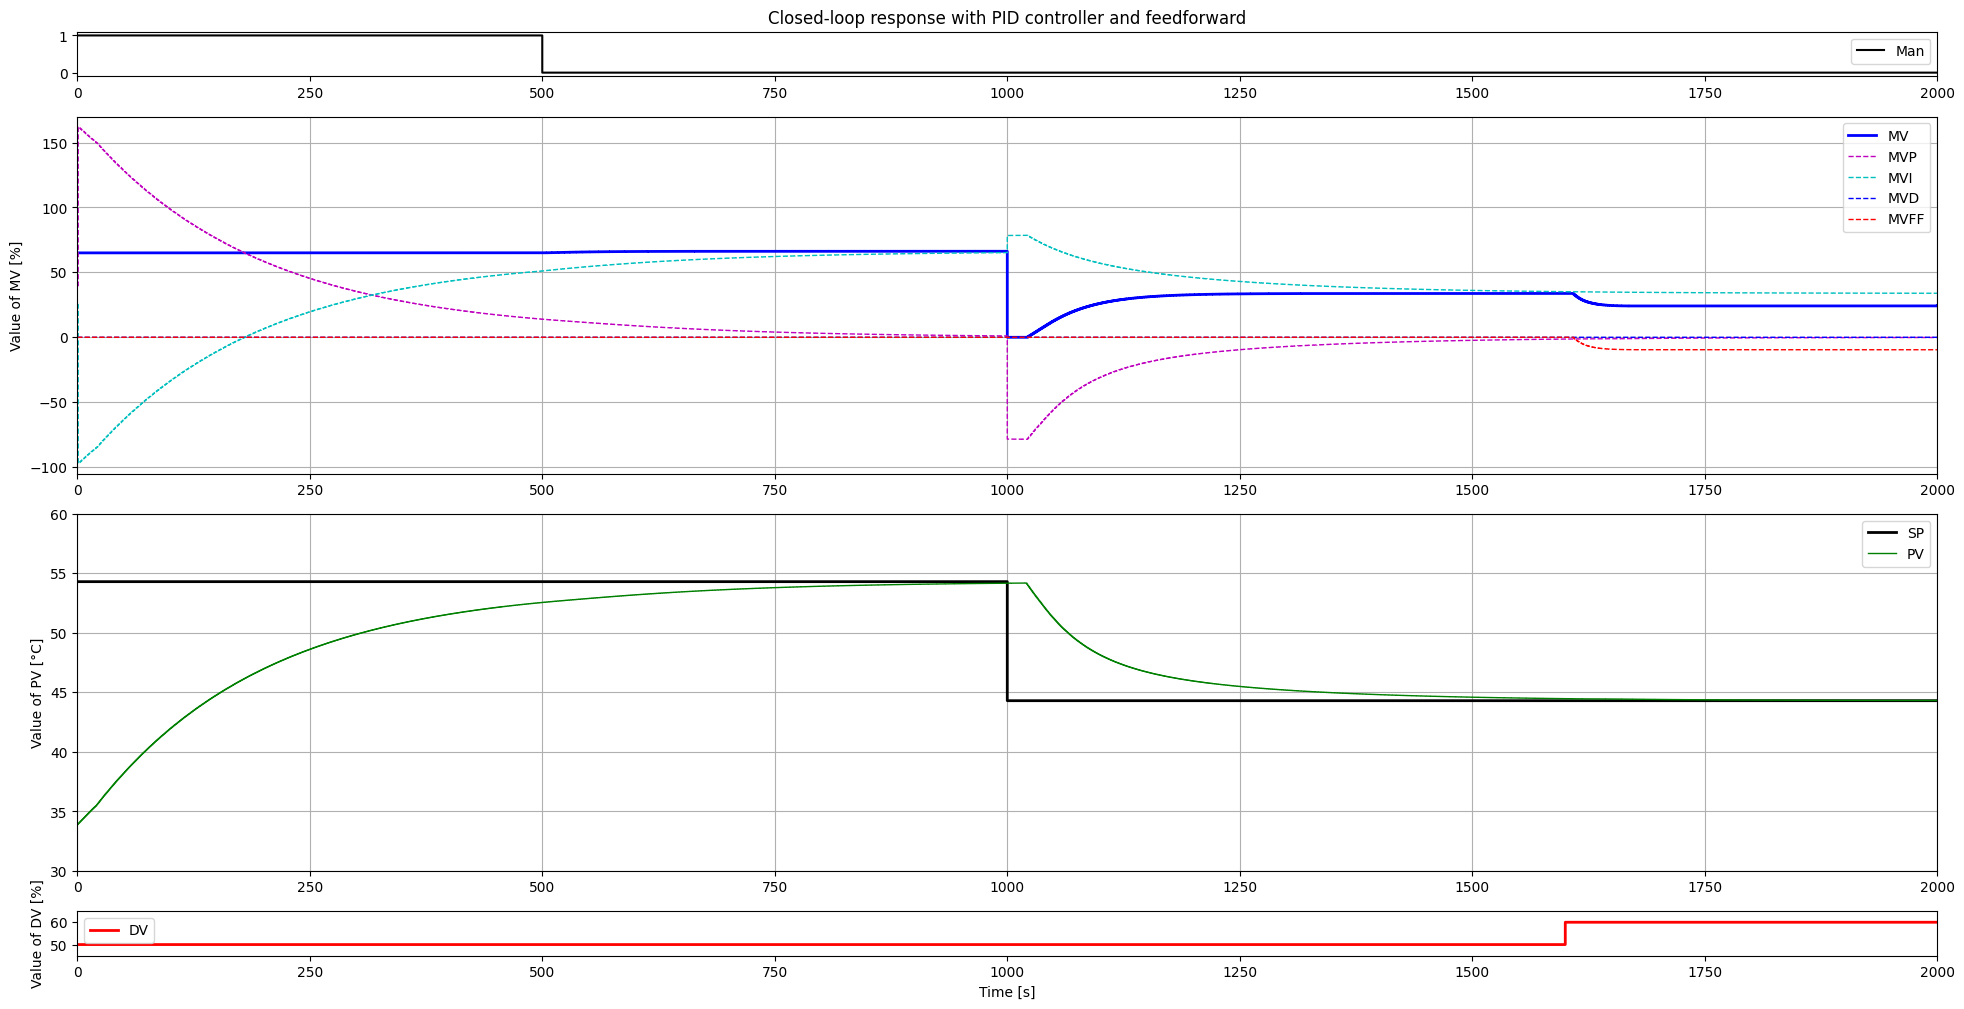
\includegraphics[width=\textwidth]{../Plots/Simulation_scenario_7_gamma=0.3.png}
        \caption{$\gamma = 0.3$}
    \end{subfigure}
    \begin{subfigure}[b]{0.48\textwidth}
        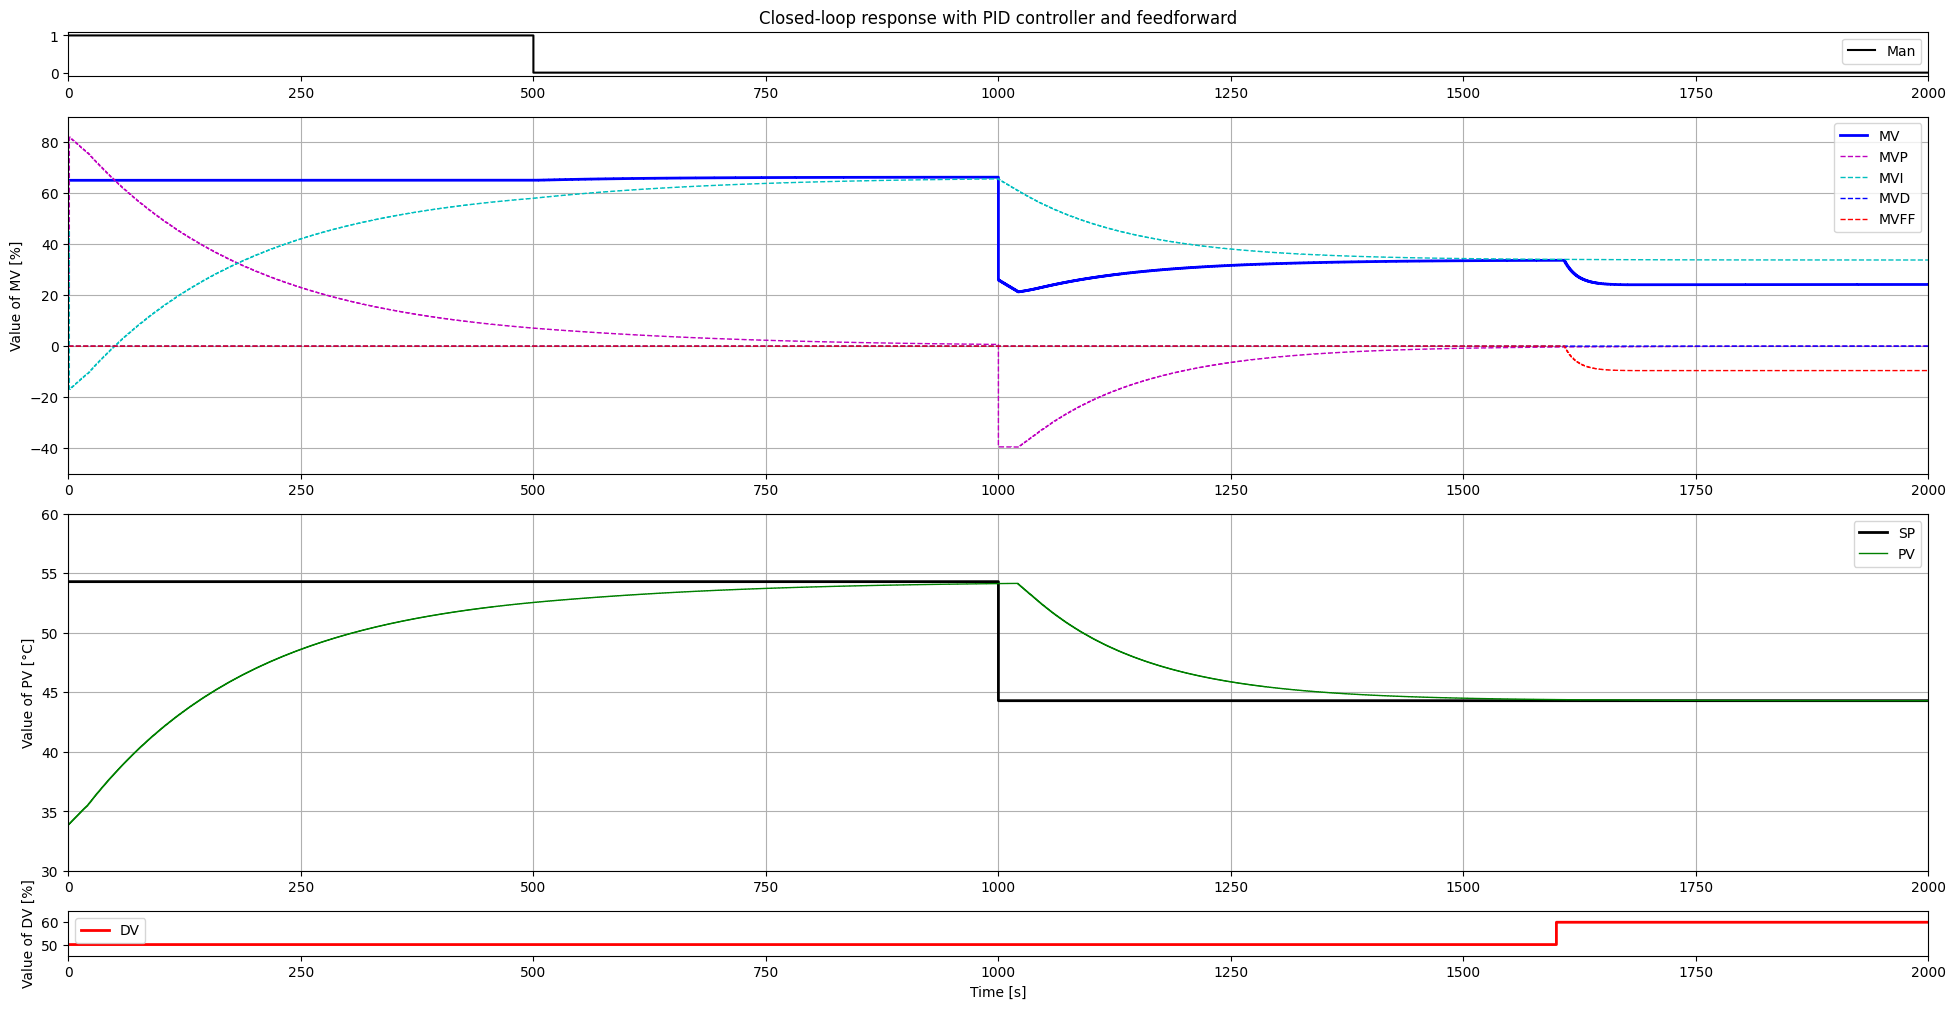
\includegraphics[width=\textwidth]{../Plots/Simulation_scenario_7_gamma=0.7.png}
        \caption{$\gamma = 0.7$}
    \end{subfigure}
    \caption{Influence de $\gamma$ sur la boucle fermée}
    \label{fig:Simulation_gamma_influence}
\end{figure}
Le paramètre $\gamma$ est utilisé dans l'optimisation IMC et fait par ce biais varier le gain du régulateur $K_C$.
\begin{equation*}
    K_C = \frac{1}{K_P} \, \frac{T_{1p} + T_{2p}}{\gamma \, T_{1p} + \theta}
\end{equation*}
Nous voyons effectivement sur la Figure \ref{fig:Simulation_gamma_influence} (a), qu'un $\gamma$ plus petit vient amplifier toutes les composantes de $MV$.
Il est alors également intéressant d'observer que l'action proportionnelle est plus grande et donc vient amener $MV$ à saturer lors du step sur la consigne.
L'action intégrale doit s'ajuster en augmentant sa valeur.\\
En se focalisant sur la phase transitoire de $PV$ lorsque le step est appliqué sur $SP$, nous pouvons noter une différence de temps de montée entre les deux simulations.
Le $\gamma$ plus petit arrive plus rapidement à 90\% de la valeur en régime établi.
Cela permet de confirmer le caractère plus aggressif du régulateur lorsque $\gamma$ est plus petit.